\documentclass[12pt,a4paper]{report}
\usepackage[T1]{fontenc}
\usepackage[utf8]{inputenc}
\usepackage{charter}
\usepackage{ngerman}
\usepackage[left=2cm,right=2cm,top=2cm,bottom=2cm]{geometry}
\usepackage{amsmath}
\usepackage{graphicx}

\begin{document}

	\noindent
	\Large
	Elektrische und mechanische Schwingungen
	\large
	\noindent
	\paragraph{a)}
	\begin{enumerate}
		\item Phase: Der Ball hat die höchste potentielle Energie erreicht.
		\item Phase: Der Ball bewegt sich und ein Teil der potentiellen Energie wird in kinetische Energie umgewandelt. Gleichzeit entsteht ein Magnetfeld.
		\item Phase: Der Ball kommt auf der anderen Seite an, die Pole werden vertauscht und der Ball hat die höchste potentielle Energie, die allerdings im Vergleich zum Anfang in die entgegengesetzte Richtung geht.
		\item Phase: Umkehrung der 2. Phase
		\item Phase: Umkehrung der 3. Phase
	\end{enumerate}
	\paragraph{LC-Kreis}
	\begin{enumerate}
		\item Phase: Aufladung
		\item Phase: Entstehung / Aufbau des Magnetfeldes
		\item Phase: Selbstinduktion
		\item Phase: Umgekehrtes Magnetfeld
		\item Phase: Umkehrung der 3. Phase
	\end{enumerate}
	\paragraph{b)}
	Im mechanischen Analogon ist die Kraft die Größe, die mit der Stromstärke vergleichbar ist.
	Dies liegt daran, dass sowohl die Stromstärke in einem elektrischen Stromkreis als auch die Kraft in einem mechanischen System die Intensität der Energieübertragung oder -bewegung darstellen.
	\paragraph{c)}
	\begin{itemize}
		\item $E_{pot} \to$ 	
		\item $E_{kin} \to$ magnetische Energie 
	\end{itemize}
	\paragraph{d)}
	\paragraph{e)} \mbox{} \\
	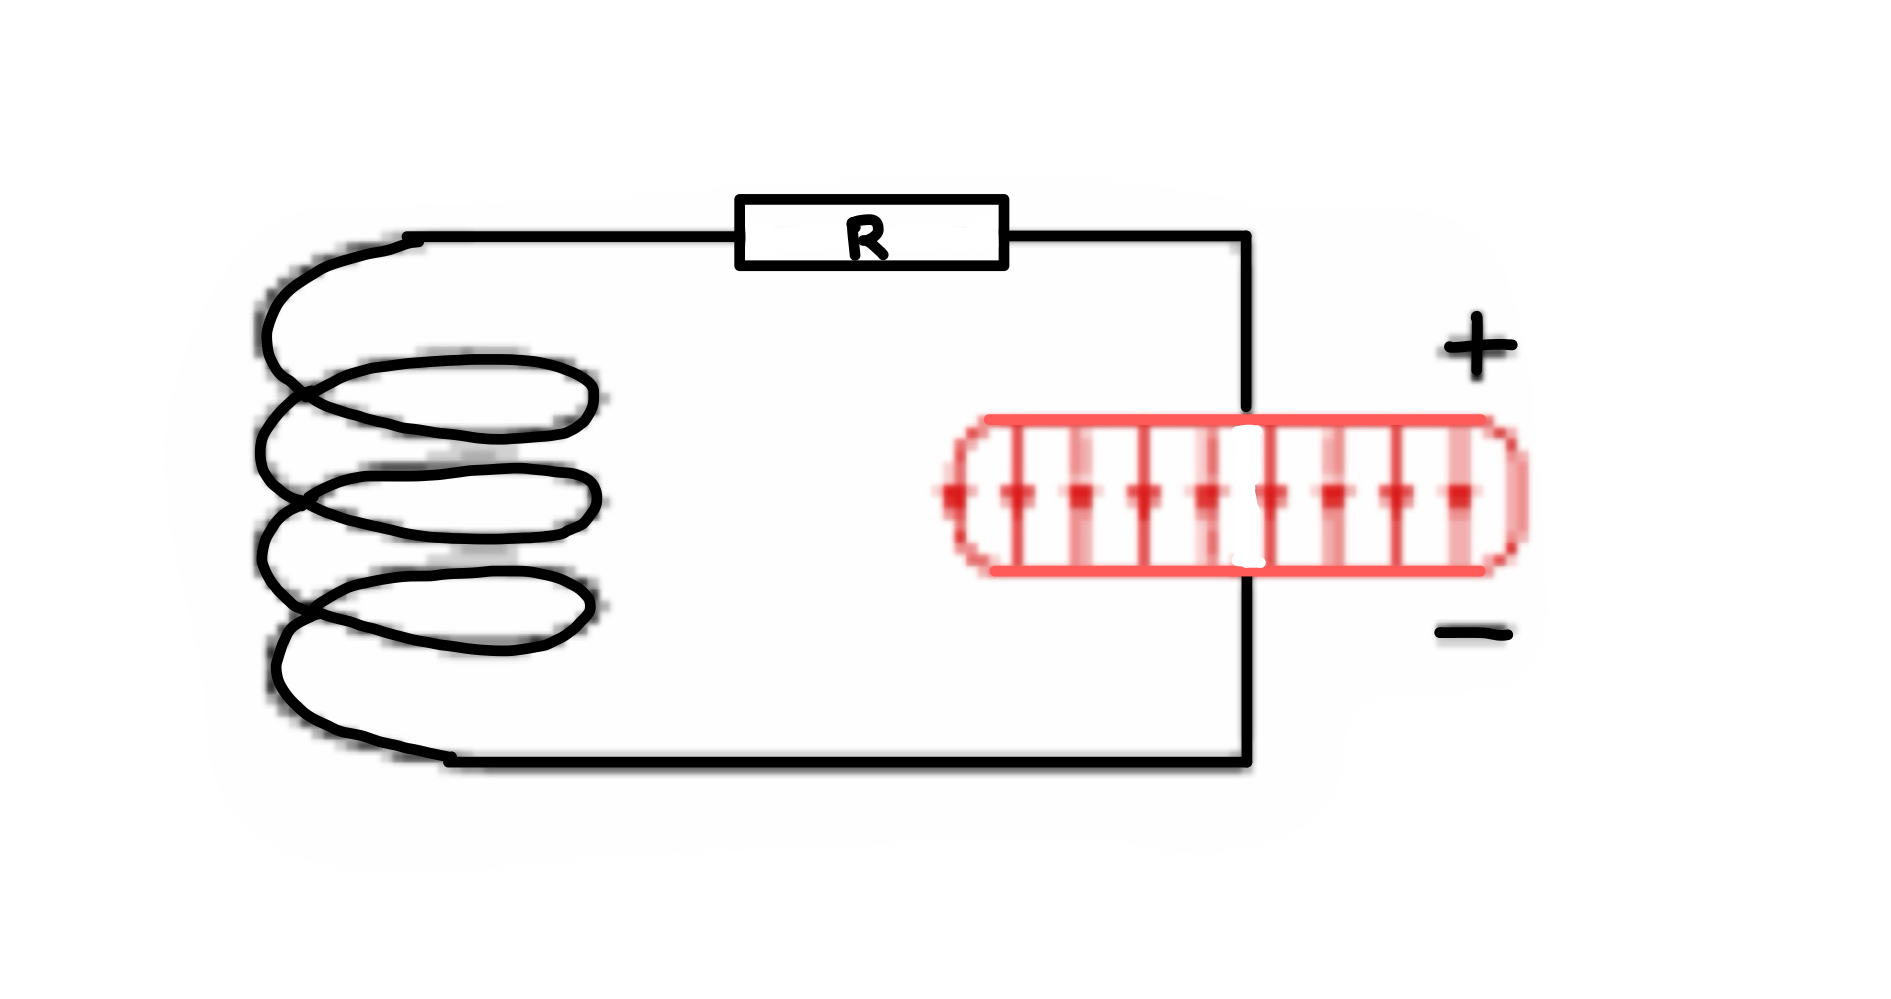
\includegraphics[width=7.5cm]{JPEG-Bild-4D19-A018-AA-0.jpeg}
	\paragraph{f)}
\end{document}